%\title{Reporte de reporte 1}
\documentclass[12pt,letterpaper]{article}     % Tipo de documento y otras especificaciones
\usepackage[utf8]{inputenc}                   % Para escribir tildes y eñes
\usepackage[spanish]{babel}                   % Para que los títulos de figuras, tablas y otros estén en español
\addto\captionsspanish{\renewcommand{\tablename}{Tabla}}					% Cambiar nombre a tablas
%\addto\captionsspanish{\renewcommand{\listtablename}{Índice de tablas}}		% Cambiar nombre a lista de tablas
\usepackage{geometry}                         
\geometry{left=18mm,right=18mm,top=21mm,bottom=21mm} % Tamaño del área de escritura de la página
\usepackage{ucs}
\usepackage{amsmath}      % Los paquetes ams son desarrollados por la American Mathematical Society
\usepackage{amsfonts}     % y mejoran la escritura de fórmulas y símbolos matemáticos.
\usepackage{amssymb}
\usepackage{graphicx}     % Para insertar gráficas
\usepackage[lofdepth,lotdepth]{subfig}	% Para colocar varias figuras
\usepackage{unitsdef}	  % Para la presentación correcta de unidades
\usepackage{pdfpages}   %incluir paginas de pdf externo, para los anexos
\usepackage{appendix}   %para los anexos
\renewcommand{\unitvaluesep}{\hspace*{4pt}}	% Redimensionamiento del espacio entre magnitud y unidad
\usepackage[colorlinks=true,urlcolor=blue,linkcolor=black,citecolor=black]{hyperref}     % Para insertar hipervínculos y marcadores
\usepackage{float}		% Para ubicar las tablas y figuras justo después del texto
\usepackage{booktabs}	% Para hacer tablas más estilizadas
\batchmode
\bibliographystyle{plain} 
\pagestyle{plain} 
\pagenumbering{arabic}
\usepackage{lastpage}
\usepackage{fancyhdr}	% Para manejar los encabezados y pies de página
\pagestyle{fancy}		% Contenido de los encabezados y pies de pagina
\usepackage{multicol}   % Para varias columnas

%---------------------------Definición del environment resumen---------------------------
\newcounter{resumen}
\setcounter{resumen}{0}
\def\theejemplo{\thechapter.\arabic{resumen}}

\newenvironment{resumen}
{	
	\begin{center}
	\begin{minipage}[t]{500 pt}
	\vspace{5mm}
	\emph{\textbf{Resumen}}
	\\[-2mm]
	\line(1,0){500}
	\\[-4.25 mm]
	\line(1,0){500}
	\\
}
{
	\normalsize
	\\[2mm]
	\footnotesize\textbf{Palabras clave: \footnotesize\@palabras}
	\\[-2mm]
	\line(1,0){500}
	\\[0.5cm]
	\end{minipage}
	\end{center}
}

% -------------------- Para las palabras clave -------------- %
\def\palabras#1{\gdef\@palabras{#1}}

%%%%%%%%%%%%%%%%%%%%%%%%%%%%%%%%%%%%

\lhead{Control I}
\chead{}
\rhead{Análisis de un sistema de primer orden}	% Aquí va el numero de experimento, al igual que en el titulo
\lfoot{Departamento de Ingeniería electrónica}
\cfoot{\thepage\ de \pageref{LastPage}}
\rfoot{Tecnológico Nacional de México}


\author{Luz Vanessa Pacheco Medina, 14121133 \\ Martha Yepez Chavez, 12121166 \\ {\small Grupo A}\\ Profesor: Gerardo Marx Chavez Campos  \vspace*{3.0in}}
\title{Tecnólogico Nacional de México\\Campus Morelia\\{\small Departamento de Ingeniería Electrónica\\Control I\\\vspace*{0.55in} Reporte De Laboratorio}\\ Análisis de un sistema de primer orden \vspace*{1.35in}}
\date{27 de octubre del 2017}  				

%%%%%%%%%%%%%%%%% PALABRAS CLAVE 
%\palabras{LateX, TINA, Filtros Pasivos}
%%%%%%%%%%%%%%%%%
% Se escriben después del resumen y sintetizan los conceptos fundamentales del experimento a modo de etiquetas


%%%%%%%%%%%%%%%%
\begin{document}	% Inicio del documento
%%%%%%%%%%%%%%%%

\pdfbookmark[1]{Portada}{portada} 	% Marcador para el título

\maketitle							% Título


\tableofcontents
\newpage
\listoffigures
%\listoftables

\newpage
\section{Introducción}
%%%%%%%%%%%%%%%%%%%
Para un sistema lineal función de párametros constantes,la función de transferencia se define como el cociente entre la transformada de Laplace de la señal de salida Y(s) y  la transformada de Laplace de la señal de entrada U(s),suponiendo todas las condiciones nulas. 



Se denominan polos a las raíces del denominador de la función de transferencia, y ceros a las raíces del numerador. El orden de la función de transferencia coincide con el grado del polinomio característico A(s), y es también el orden de la ecuación diferencial asociada.

Un sistema es de orden mínimo si no hay cancelaciones entre polos y ceros en la función de transferencia. 

Una función de transferencia es propia si el orden del numerador es menor o igual que el del denominador. Si es menor, es estrictamente propia. La mayoría de los sistemas reales tienen funciones de transferencia propias. 

Solo es aplicable a sistemas descritos por ecuaciones diferenciales lineales invariantes en el tiempo, depende de las carcteristicas del sitema y no de la magnitud y tipo de entrada, además no proporciona información de la estructura interna del sistema.
\begin{figure}[h!]
\centering
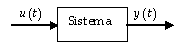
\includegraphics[width=3in]{funciones}
\caption{Relación de una función de transferencia}
\end{figure}

Ventajas de la función de transferencia:


1.- Es una representación compacta de un sistema lineal como cociente del polinomio en s.

2.-Permite predecir la forma de las señales sin necesidad de resolver la escuación diferencial.

3.-Tiene una interpretación inmediata en la fecuencia: s=jw 

4.-Es una propiedad del sistema: Independiente de la magnitud y la naturaleza de la señal de entrada.

5.- Si se desconoce la ecuación diferencial que describe el sistema, se puede obtener su funcion de transferencia de forma experimental, excitando al sistema con entradas conocidas y estudiando la respuesta.

\subsection*{Diagramas de bloques}
La relación causa y efecto  de la funcion de transferencia, permite representar las relaciones de un sistema por medios digrámaticos.

Los diagramas de bloques de un sistema son bloques operacionales y unidireccionales que representan la función de transferencia de las variables de interés.


%%%%%%%%%%%%%%%%%%%


%%%%%%%%%%%%%%%%%%%
\section{Metodología}
%%%%%%%%%%%%%%%%%%%

\begin{figure}[h!]
\centering
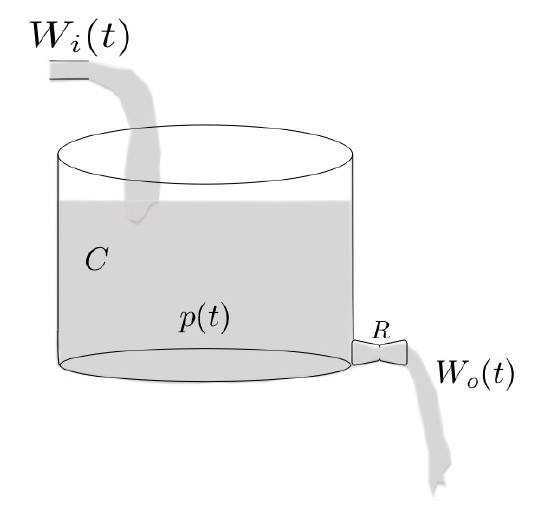
\includegraphics[width=3in]{6}
\caption{Sistema hidráulico}

\end{figure}
Se describen los términos del diagrama para llevar a obtener la ecuación del balance de la energía en (\ref{eq:ej}):
\begin{equation}\label{eq:ej}
E_{GEN} + E_{IN} = E_{AC} + E_{OUT}
\end{equation}
Donde:

EGEN: Energía generada.\\
EIN: Energía de entrada.\\
EAC: Energía acumulada.\\
EOUT: Energía de salida.\\\\
Se iguala la salida a 
\[
w_{o}(t)=Rh(t) -> rgh(t)/R
\]
Se obtiene la siguiente ecuación de balance de energía:
\begin{equation}\label{eq:ej1}
w_{i}(t) = A\frac{dh(t)}{dt} +\frac{rgh(t)}{R} 
\end{equation}

Donde:
h(t)=altura
C: Es la capacitancia.
R: La resistencia hidráulica.
A: El área.
wi: La entrada.
Se obtiene el siguiente circuito equivalente del sistema hidráulico

\begin{figure}[h!]
\centering
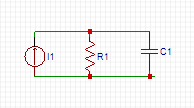
\includegraphics[width=3in]{7}
\caption{Circuito equivalente del sistema hidráulico}
\end{figure}
Del sistema mostrado anteriormente se obtiene la siguiente función de transferencia:
\begin{equation}\label{eq:ej2}
w_{i}(t) = \frac{h(t)}{R} +C\frac{dh(t)}{dt} 
\end{equation}
Tomando en cuenta que R=R/rg y C=A
Se aplica LAPLACE
\begin{equation}\label{eq:ej3}
w_{i}(S) = \frac{H(S)}{R} +CSH(S)+H(0) 
\end{equation}
Factorizando  se obtiene la función de transferencia siguiente:
\begin{equation}\label{eq:ej4}
G(S) = \frac{\frac{1}{C}}{S+\frac{1}{RC}}
\end{equation}
Utilizando la siguiente ecuación se desarrolla el sistema genérico para obtener la función de transferencia introduciendo sólo variables a, b y c:
\begin{equation}\label{eq:ej5}
G(S) = \frac{bS+C}{S+a}
\end{equation}
Se expresa en fracciones parciales H(S) para obtener los valores de A y B
\begin{equation}\label{eq:ej6}
H(S) = w_{i}(S)\frac{bS+C}{S+a}
\end{equation}
\begin{equation}\label{eq:ej7}
H(S) = \frac{A}{S}+\frac{B}{S+a}
\end{equation}
Se multiplica 1/S (función impulso) por la ecuación para aplicar fracciones parciales
\begin{equation}\label{eq:ej8}
H(S) =\frac{1}{S}*\frac{bS+c}{S+a}
\end{equation}
Se iguala el numerador con las fracciones parciales
\begin{equation}\label{eq:ej9}
bS+c = \frac{A}{S}+\frac{B}{S+a}
\end{equation}
Se distribuyen los valores para obtener las ecuaciones:
\begin{equation}\label{eq:ej10}
bS+c = AS+Aa+BS
\end{equation}
Se tienen las siguientes ecuaciones:\\
A + B = b\\
A a = c\\
Se despeja A:\\
A = c/A\\
Se despeja B:\\
B = b - c/a
La función de transferencia es:
\begin{equation}\label{eq:ej11}
H(S) = \frac{c}{a}S + \frac{b-\frac{c}{a}}{S+a}
\end{equation}
Respecto al tiempo, ya que u(t)=1:
\begin{equation}\label{eq:ej11}
h(t) = \frac{c}{a} + (b-\frac{c}{a})e^{-at}
\end{equation}
\subsection*{Cálculos Para Obtener wi=wo, wi<wo, wi>wo}
\begin{equation}\label{eq:ej12}
w_{i}(t) = \frac{h(t)}{R} + \frac{Cdh(t)}{dt}
\end{equation}
Se requiere wi=wo utilizando la ecuación de la energía, sustituimos valores a la entrada y la salida, recordando que wo es la corriente del capacitor.\\
1=1+h(t)/R\\
h(t)=1\\
R=0.\\

Si se requiere que wi>wo\\
2=1+h(t)/R
Se da un valor a la entrada mayor\\
R=h(t)\\
La salida aumentará de cero a uno.\\
Si se requiere que wo>wi\\
1=2+h(t)/R
Se da un valor a la entrada menor generando un R=-h(t)\\
La salida decrecerá de uno a cero.\\
%%%%%%%%%%%%%%%%%%%%%%%%%%%%%%%%%%

%%%%%%%%%%%%%%%%%%%%%%%%%%%%%%%%%%
\subsection{Código de los programas}
\begin{table}[htbp]
\begin{center}
\begin{tabular}{|l|l|}
\hline
vector=input("Ingrese el vector de coeficientes: ")\\

a=vector(1);\\
b=vector(2);\\
c=vector(3);\\

A=(c/a);\\
B=(b-(c/a));\\
t=0:0.01:15;\\ 
fun=(A+B*exp(-a*t));\\
plot(t,fun) \\
\hline 

\end{tabular}
\caption{código generado para la práctica}
\label{cód1}
\end{center}
\end{table}

\begin{table}[htb]
\begin{center}
\begin{tabular}{|l|l|}
\hline
s=s% //The quicker alternative to using s=poly(0,'s')\\
//Gain and time constant\\
k= 1;\\
tau=0.001;\\
simpleSys=syslin('c', k/(1+tau*s))\\
t=0:0.01:15;\\
y=csim('step', t, simpleSys)\\
plot(t,y)\\
\hline 

\end{tabular}
\caption{código de Scilab ejemplo}
\label{cód2}
\end{center}
\end{table}

\section{Resultados y Discusión}
Si la entrada y salida son iguales el contenedor se mantiene con un líquido constante.\\
\subsection{Entrada igual a la salida}
\begin{figure}[h!]
\centering
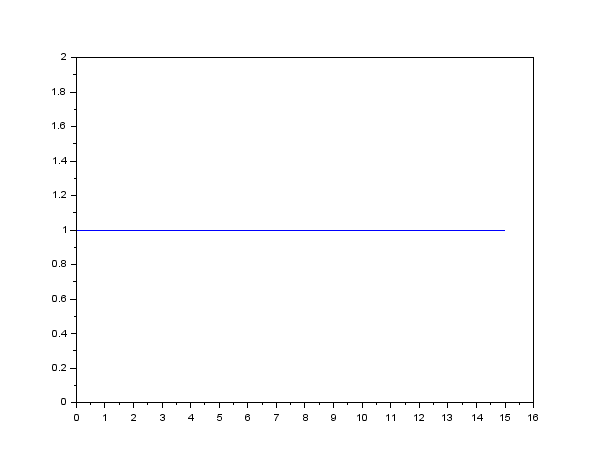
\includegraphics[width=3in]{1}
\caption{Entrada igual a la salida, función impulso}
\end{figure}
\begin{figure}[h!]
\centering
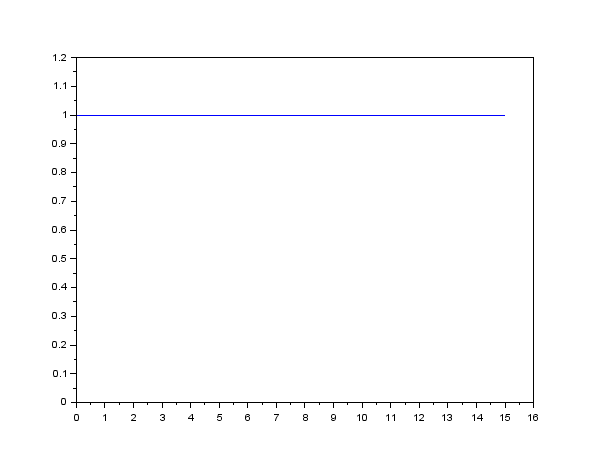
\includegraphics[width=3in]{4}
\caption{Entrada igual a la salida, código Scilab}
\end{figure}
\textbf{Observación:}
La relación de la salida con la entrada para que ambos sean iguales debe ser uno, para ello a, b y c deben tomar el valor de uno, manteniendose en un valor de uno, en la función de Scilab que se proporcionó se cambió el valor de k al que corresponde a  R=1, poniendo también un valor cercano a Tau.\\
Se puede ver que el tanque se mantiene constante tanto en la función de Scilab y la de función impulso obtenida.\\\\

\subsection{Salida menor que la entrada}
\begin{figure}[h!]
\centering
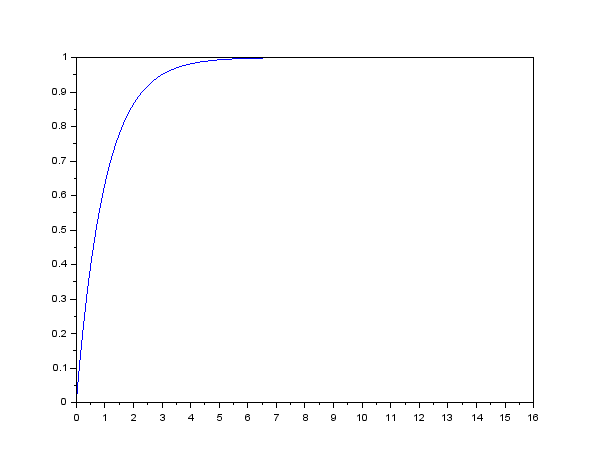
\includegraphics[width=3in]{2}
\caption{Salida menor que la entrada con función impulso}
\end{figure}
\begin{figure}[h!]
\centering
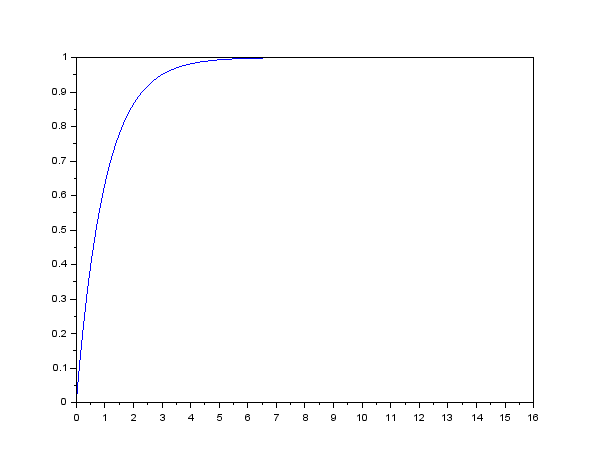
\includegraphics[width=3in]{3}
\caption{Salida menor que la entrada con función impulso}
\end{figure}
\textbf{Observación:}
En el código genérico se agregaron los valores de a=1, b=0 y c=1,
Se puede ver que el tanque se va llenando, y llega hasta uno comovalor máximo, se comprobó con el código de Scilab mostrando la misma exponencial creciente con un valor de 1 en R y en Tau, se buscaron las relaciones entre las dos funciones de transferencia para encontrar valores a la resietencia y Tau que nos mostraran la misma respuesta en el código genérico de la respuesta impulso con los valores a, b y c.\\\\

\subsection{Salida mayor a la entrada}

\textbf{Observación:}
En el código genérico se agregaron los valores de a=1, b=0 y c=-1,
Se puede ver que el tanque se va vaciando, ya que nuestra condición inicial es cero se observa que decrece de 0 a -1, sin embargo si existiera una cocndición inicial de 1, ya que se considere el tanque lleno el sistema se descarga de 1 a cero, es cuestión de apreciación, en el código de Scilab se cambia el valor de R=-1 por la k.\\
\begin{figure}[h!]
\centering
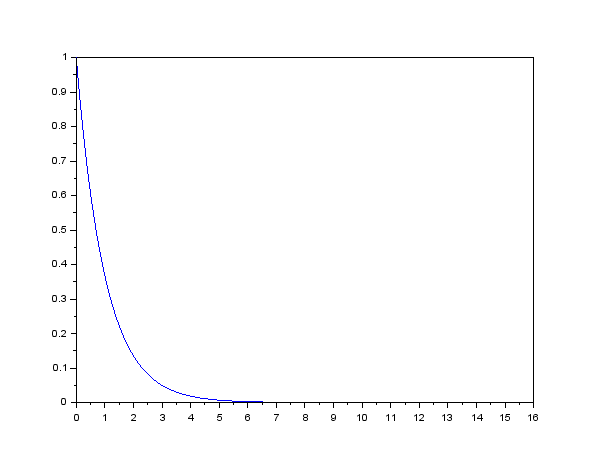
\includegraphics[width=3in]{5}
\caption{Salida mayor que la entrada con función impulso}
\end{figure}
\begin{figure}[h!]
\centering
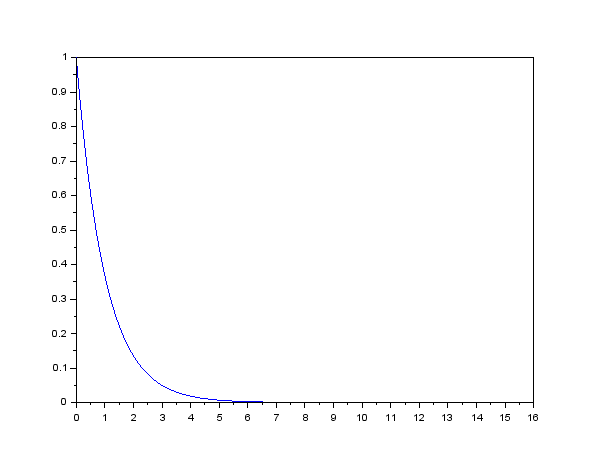
\includegraphics[width=3in]{8}
\caption{Salida mayor que la entrada con función de scilab}
\end{figure}

\newpage
%%%%%%%%%%%%%%%%%%%%%%%
\section{Conclusiones}
Martha Yepez Chavez:\\
 En conclusión  después de analizar la función de transferencia con ayuda de scilab  hemos comprendido el comportamiento de diferentes sistemas utilizando el modelo general para solucionarlos.

A nosotros como estudiantes el utilizar un software de este tipo nos fácilita el comprender desde el punto matemático cual es el comportamiento en respuesta a otra función.

Gracias a las funciones de scilab pudimos visaulizar de manera gráfica el comportamiento de los sistemas. 

Además el desarrollar el algoritmo para la resolución general, nos ayudo para reforzar los conceptos vistos en las clases anteriores y tener ya un modelo para resolver futuros sistemas de primer orden.\\\\
Luz Vanessa Pacheco Medina:\\
Las funciones de transferencia tienen gran utilidad en la representación de distintos sistemas, se pudieron comprobar sistemas hidráulicos en la práctica y mecánicos en la teoría, sin embargo, una presentación de ellos mediante circuitos eléctricos tranen grandes ventajas a la hora de representar algunas partes como elementos pasivos (capacitores, inductores y resistencias), para ello es muy complejo si se manejan resoluciones con ecuaciones diferenciales, así se implementa la transformada de Laplace que convierte a todo sistema en una forma más fácil de observar. \\
Se utilizáron dos modelos distintos en Scilab para llevar a cabo la graficación del sistema hidráulico, una forma con un sistema específico del sistema hidráulico, y otro generalizado para introducir sólo los valores de tres coeficientes que se ordenarían en una forma general y nos darían directamente la respuesta del sistema.

%%%%%%%%%%%%%%%%%%%%%%%


%%%%%%%%%%%%%%
% Bibliografía
%%%%%%%%%%%%%%

\newpage

El formato recomendado para la bibliografía es el APA. El siguiente es un ejemplo:

\begin{thebibliography}{}
\bibitem[Apuntes, 2012]{Funciones de transferencia} \emph{http://ocw.uc3m.es/ingenieria-de-sistemas-y-automatica/senales-y-sistemas/temas/tema-4-funcion-de-transferencia} consultado el 26/10/2017.

\bibitem[Ingeniería de control moderna, 1998]{} Katsuhiko Ogata (1974). \emph{Ingeniería de control moderna}. USA:  Pearson Prentice Hall, 4th Edition.



\end{thebibliography}

\newpage


%%%%%%%%%%%%%%
\end{document}
%%%%%%%%%%%%%%